%%%%%%%%%%%%%%%%%%%%%%%%%%%%%%%%%%%%%%%%%
% Invoice Template
% LaTeX Template
% Version 1.0 (3/11/12)
%
% This template has been downloaded from:
% http://www.LaTeXTemplates.com
%
% Original author:
% Trey Hunner (http://www.treyhunner.com/)
%
% License:
% CC BY-NC-SA 3.0 (http://creativecommons.org/licenses/by-nc-sa/3.0/)
%
% Important note:
% This template requires the invoice.cls file to be in the same directory as 
% the .tex file. The invoice.cls file provides the style used for structuring the
% document.
%
%%%%%%%%%%%%%%%%%%%%%%%%%%%%%%%%%%%%%%%%%

%----------------------------------------------------------------------------------------
%	DOCUMENT CONFIGURATION
%----------------------------------------------------------------------------------------

\documentclass{invoice} % Use the custom invoice class (invoice.cls)

\usepackage{natbib}
\usepackage{graphicx}
\usepackage{wrapfig}



\def \tab {\hspace*{3ex}} % Define \tab to create some horizontal white space

\begin{document}

%----------------------------------------------------------------------------------------
%	HEADING SECTION
%----------------------------------------------------------------------------------------

\begin{figure}
	\centering
	
	\includegraphics[width=0.2\textwidth]%
	{idea161.jpg}% picture filename
    
    %\caption{ \hfil{\Huge\bf IDEA 1.61}\hfil}
    
\end{figure}

%\hfil{\Huge\bf IDEA 1.61}\hfil % Company providing the invoice

%\begin{figure}
%	
\includegraphics[width=0.1\textwidth]{idea161.jpg}
%\end{figure}


%\bigskip
%\break % Whitespace
\hrule % Horizontal line

Coyoacán \hfill 55-2525-8429 \\ % Your address and contact information
Ciudad de México, México \hfill contacto@idea161.org
\\ 
{\bf Note for: Mich Gb} \\
\tab   % Invoice recipient
%\tab Generico \\ % Recipient's company

{\bf Date:} \\
\tab \today % Invoice date

%{\bf Expira:} \\
%\tab  \\ % Invoice date
%----------------------------------------------------------------------------------------
%	TABLE OF EXPENSES
%----------------------------------------------------------------------------------------

\begin{invoiceTable}

%\feetype{Impresión 3D} % Fee category description

%\hourrow{Base}{67}{0.75}



\feetype{Impresiones 3D}

\hourrow{6mm-hexagonal-gear}{12}{0.65}
\hourrow{6mm-hexagonal-insert}{3}{0.65}
\hourrow{big-intermediate-gear-and-washer}{69}{0.65}
\hourrow{BIG-Spur-Gear-16-teeth}{71}{0.65}
\hourrow{bobin-gear-v1}{159}{0.65}
\hourrow{double-end-driving-gear}{28}{0.65}
\hourrow{hex-bolt-gear}{13}{0.65}


\hourrow{long-driving-gear-with-key}{27}{0.65}
\hourrow{Rolling-Pin-Gear-2-Solid-Deeper-Ring}{36}{0.65}



\hourrow{Rolling-Pin-Gear-2-Solid-Deeper-Ring}{134}{0.65}
\hourrow{Spur-Gear-6-teeth}{19}{0.65}
\hourrow{v3-side-arm}{124}{0.65}

\hourrow{v3-side-arm-mirror}{134}{0.65}
\hourrow{v3-side-panel-hollow}{15}{0.65}


%\feetype{Componentes} % Fee category description



%\feetype{Servicios} % Fee category description

%\hourrow{Préstamo Cautin y Uso del espacio}{1}{35}
%------------------------------------------------

%\feetype{Accounting Services} % Fee category description

%\hourrow{October 11, 2012}{1}{80}

\subtotal % Prints a subtotal, can be used multiple times

%------------------------------------------------

%\feetype{Hosting Expenses} % Fee category description

%\feerow{Descuento 10$\%$}{-125.65} % A flat fee service, note there is no hourly rate for this

\end{invoiceTable}

%Hola
%\begin{figure}[h!]
%	\centering
%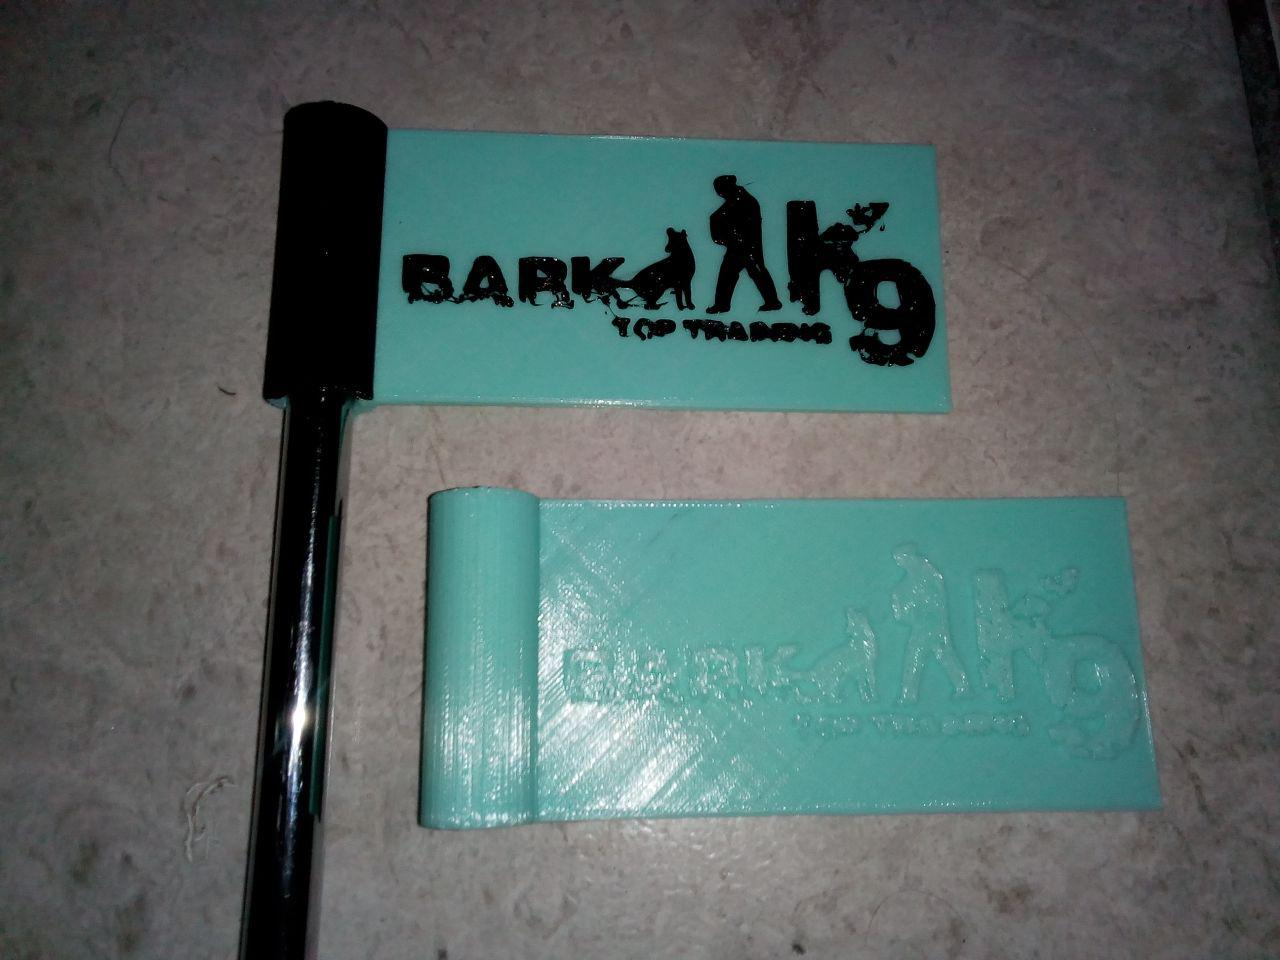
\includegraphics[width=0.3\textwidth]{bandera.png}
%\end{figure}
%----------------------------------------------------------------------------------------

\end{document}\grid
